\section{TP4: IR}
\subsection{Objectif}
Dans cette manipulation nous allons voir comment utiliser une télécommande infra rouge et un récepteur infra rouge pour controller des modules à une distance pouvant aller jusqu'a 10 metres. Nous allons donc controller une LED, la couleur d'une LED RGB ainsi qu'un moteur.
\subsection{Matériel}
\begin{itemize}
	\item Un ordinateur
	\item Un arduino Uno R3
	\item Un récepteur IR
	\item Des resistance de 10K$\Omega$
	\item Une led
	\item Une LED RGB
	\item Un Un moteur avec controlleur
\end{itemize}

\subsection{Controle d'une LED à distance}

\lstinputlisting[language=C]{Code/TP4/TP4.1/TP4.1.ino}
\begin{figure}[H]
	\centering
	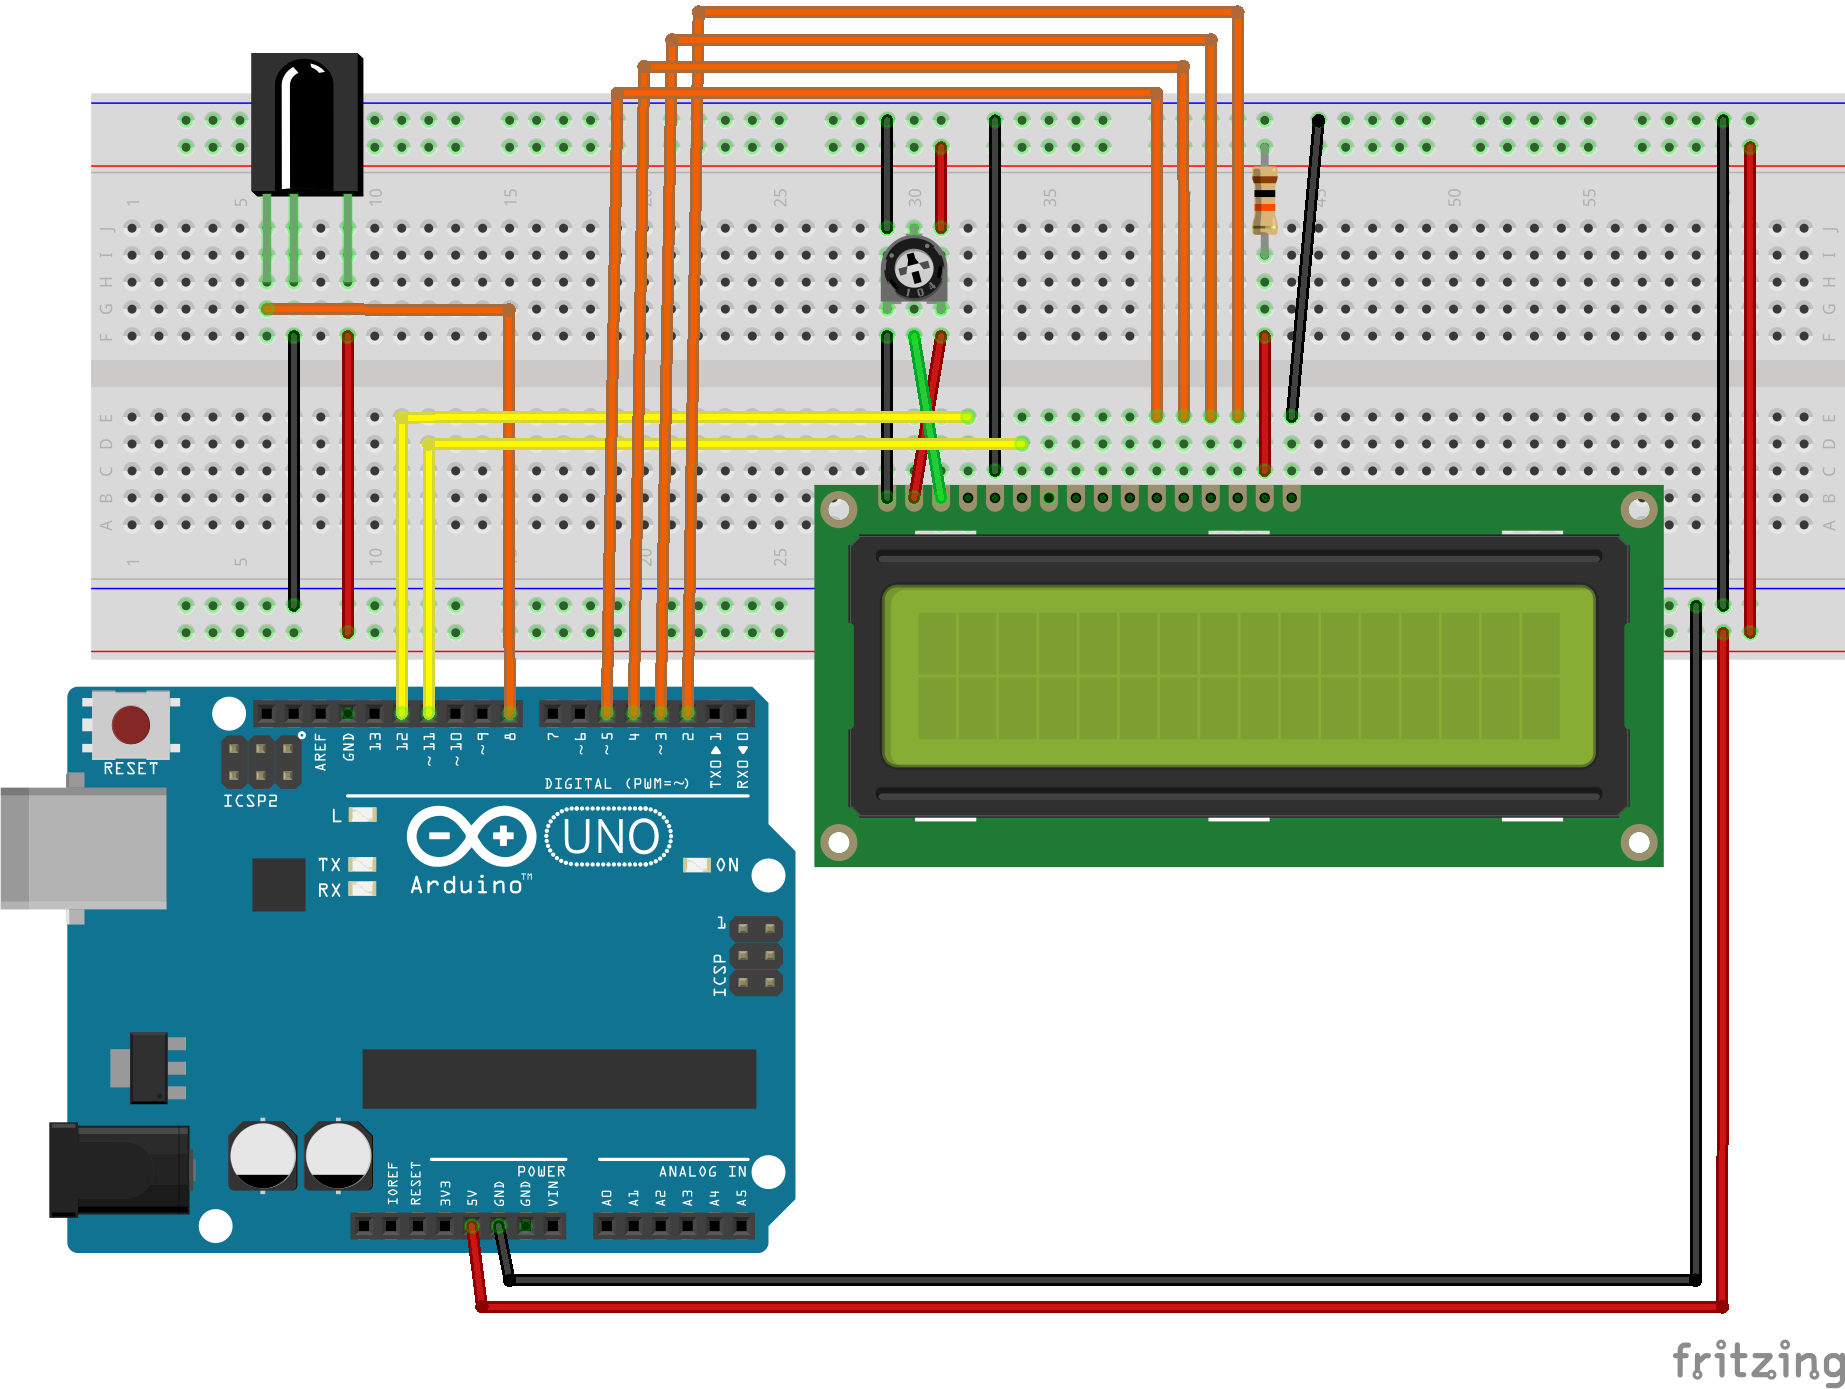
\includegraphics[height=6cm]{img/TP4-1.png}
	\caption{\label{TP4.1}Controle d'une LED}
\end{figure}


\subsection{Controle de la couleur d'une LED RGB à distance}

\lstinputlisting[language=C]{Code/TP4/TP4.2/TP4.2.ino}
\begin{figure}[H]
	\centering
	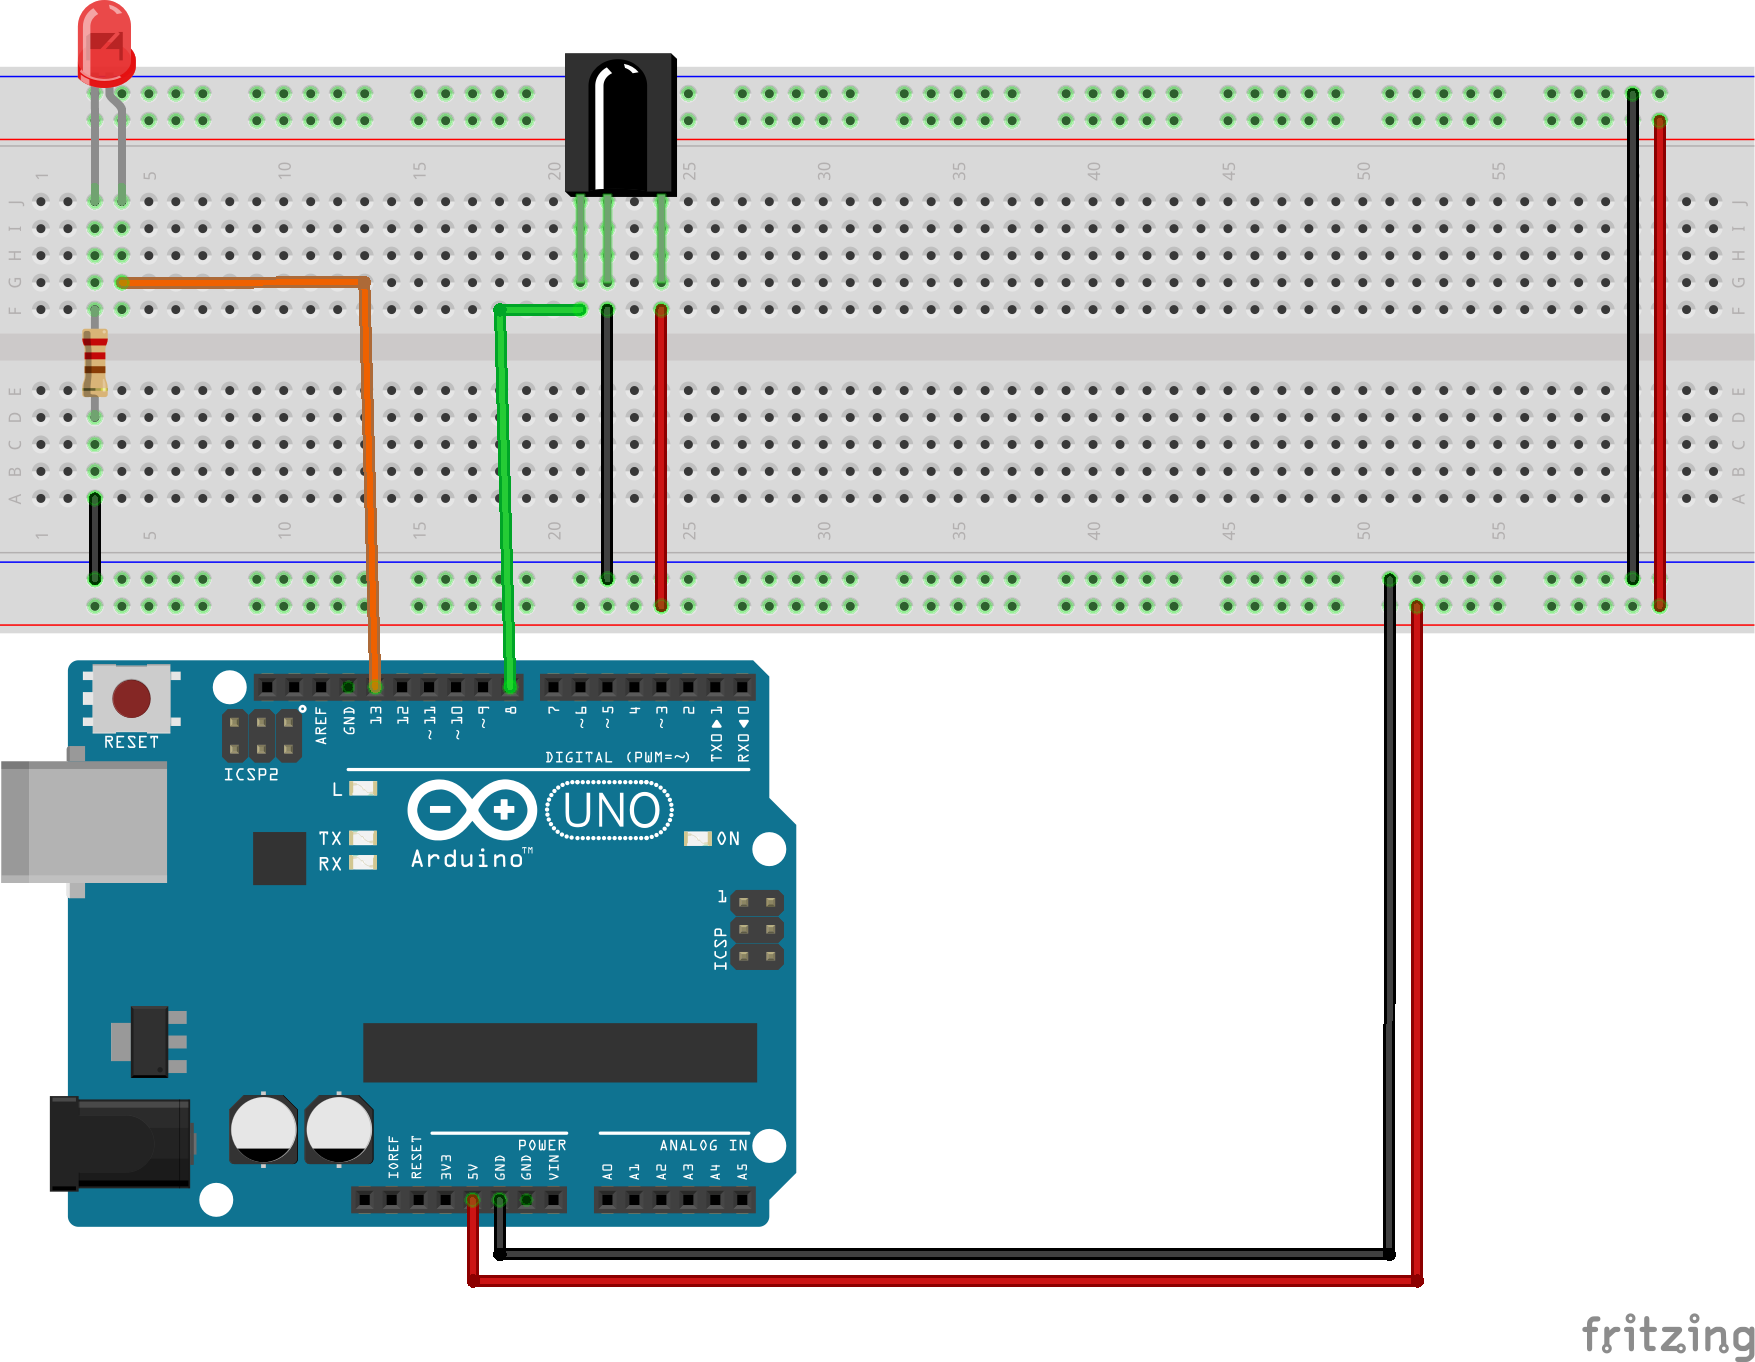
\includegraphics[height=6cm]{img/TP4-2.png}
	\caption{\label{TP4.2}Controle d'une LED RGB à distance}
\end{figure}

\subsection{Controle d'un moteur à distance}

\lstinputlisting[language=C]{Code/TP4/TP4.3/TP4.3.ino}
\begin{figure}[H]
	\centering
	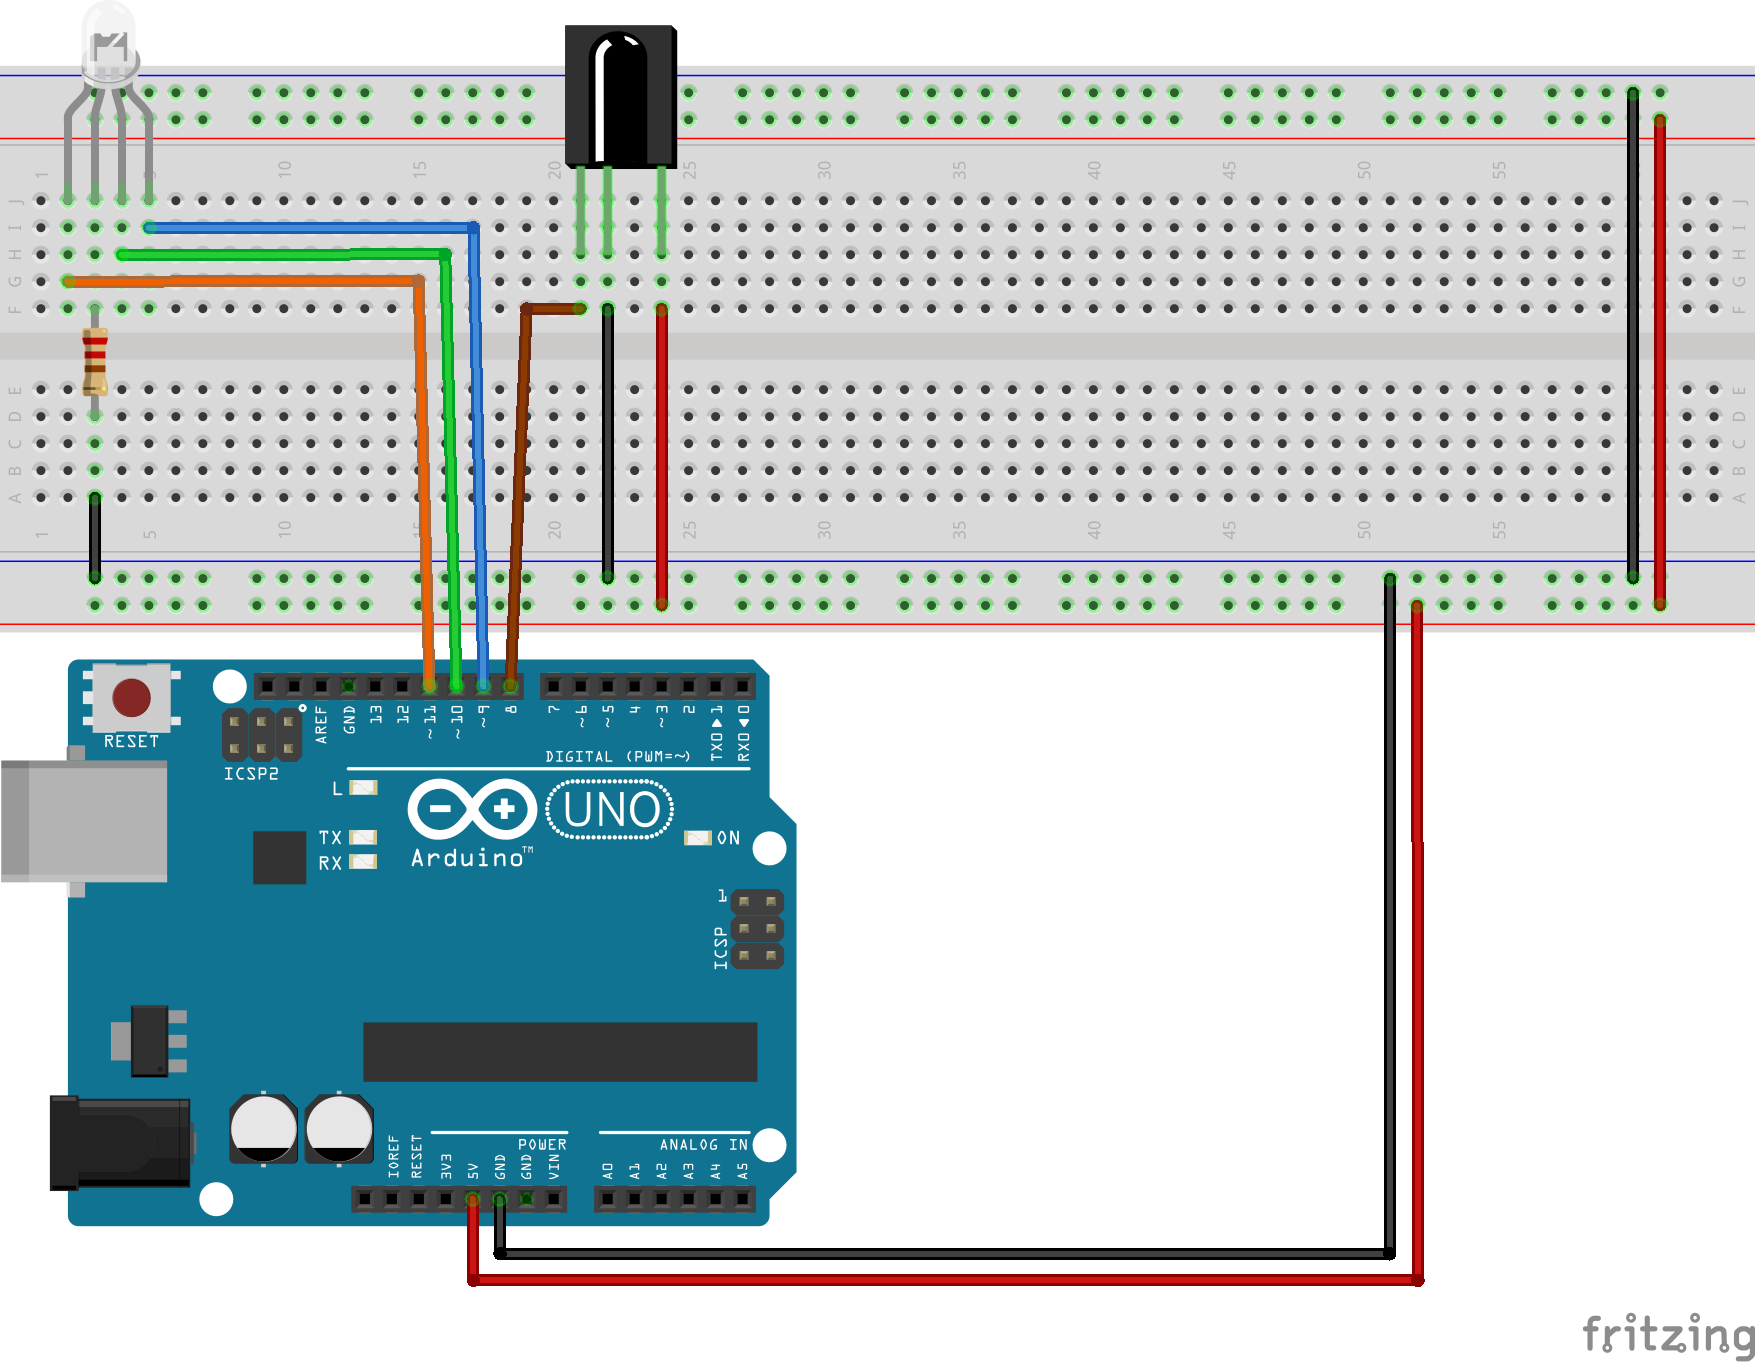
\includegraphics[height=6cm]{img/TP4-3.png}
	\caption{\label{TP4.3}Controle d'un moteur à distance}
\end{figure}

% \subsection{Joystick et matrice de LED}

% \lstinputlisting[language=C]{Code/TP3/TP3.4/TP3.4.ino}
% \begin{figure}[H]
% 	\centering
% 	\includegraphics[height=6cm]{img/TP3-4.png}
% 	\caption{\label{TP3.4}Joystick et matrice de LED}
% \end{figure}
